\section{Resolução}

\subsection{Conta Bancária}

\begin{multicols}{2}
	\lstinputlisting{../ex11/contaBancaria.h}

	\lstinputlisting{../ex11/contaBancaria.c}
\end{multicols}	
\newpage
\begin{multicols}{2}
	\lstinputlisting{../ex11/main.c}
\end{multicols}

\begin{figure}[h!]
	\centering
	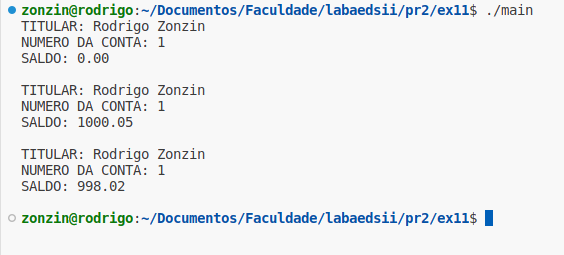
\includegraphics[width=0.7\linewidth]{q1}
	\caption{Saída}
	\label{fig:q1}
\end{figure}

\subsection{CatalogoProduto}
\begin{multicols}{2}
	\lstinputlisting{../ex12/Produto.h}
	\lstinputlisting{../ex12/CatalogoProduto.h}
\end{multicols}	

\begin{multicols}{2}	
	\lstinputlisting{../ex12/CatalogoProduto.c}
\end{multicols}	

\begin{figure}[h!]
	\centering
	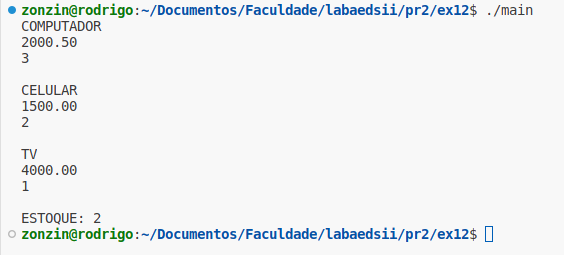
\includegraphics[width=0.7\linewidth]{q2}
	\caption{Saída}
	\label{fig:q2}
\end{figure}


\section{Análise de Complexidade}
\subsection{}
$$insercao = 8n^2$$
$$intercalacao = 64n\cdot lg(n)$$

Podemos analisar a seguinte inequação

$$insercao \geq intercalacao $$
$$8n^2 \geq 64n\cdot lg(n)$$
$$n^2 \geq 8n\cdot lg(n)$$
$$\frac{8}{n}   \geq lg(n)  \forall n \geq 44$$


\subsection{}

$f(n) = 100n^2$ \\
$g(n) = 2^n$

Portanto, 
$$ f(n) \leq g(n) $$ 
$$ 100n^2 \leq 2^n$$ 
$$lg(100n^2) \leq lg(2^n)$$
$$lg(100)+2lg(n) \leq n lg(2)$$
$$lg(100)+2lg(n) \leq n$$
$$2lg(10) + 2lg(n) \leq n$$
$$6.64 + 2lg(n) \leq n$$
É fácil perceber  que $f(n)$ é pior que $g(n) \ \forall n \in \left[ 15, \infty \right)  $ \\



\begin{flushleft}
	Sejam $f$ e $g$ duas funções de complexidade quaisquer em $\mathbb{R}$.
\end{flushleft}
\subsection{}
\begin{definition}
	Notação $O$: Limite assintótico superior
	
	$\exists c, m \in \mathbb{R^+}, |g(n)| \leq c \cdot |f(n)| \forall n>m \Rightarrow g(n) = O(f(n))$
\end{definition}
Para qualquer valor de $n \geq m$, $g$ sempre terá imagem menor que a imagem de $c \cdot f$ para tais constantes $m$ e $c$.

\subsection{}

\begin{definition}
	Notação $\Omega$: Limite assintótico inferior
	
	$\exists c, m \in \mathbb{R^+}, |g(n)| \geq c \cdot |f(n)| \forall n>m \Rightarrow g(n) = \Omega(f(n))$
\end{definition}
Para qualquer valor de $n \geq m$, $g$ sempre terá imagem maior que a imagem de $c \cdot f$ para tais constantes $m$ e $c$.

\subsection{}
A notação $O$ é capaz de descrever o ``teto" de desempenho de um algoritmo, mas não seu limite inferior. 
Dessa maneira, só é possível dizer: \textit{O tempo de execução do algoritmo A é no máximo $O(n^2)$}.

\subsection{}
$a(n) = n^2-n+500$ \\
$b(n) = 47n-47$

Fazemos, 

$$a(n) \leq b(n)$$
$$ n^2-n+500 \leq 47n-47 $$
$$n^2-48n + 453 \leq 0$$
Resolvendo para a igualdade, obtemos $n_1 = 35,09$ e $n_2 = 12,91$. Como $n$ é obrigatoriamente pertencente aos inteiros positivos, temos: \\
$$a(n) \leq b(n)  \Leftrightarrow n \in \left[ 13,35 \right] $$

\subsection{}
$\sum_{i = 0}^{N-1} \sum_{j=i}^{N} \sum_{k=1}^{j} s$\\
$= \sum_{i = 0}^{N-1} \sum_{j=i}^{N} js$\\
$= \sum_{i = 0}^{N-1}  s ( \sum_{j=i}^{N} j  - \sum_{j=1}^{i-1}j)$\\
$= s \sum_{i = 0}^{N-1}  \frac{N^2 - N}{2} $\\
$= s N  \frac{N^2 - N}{2} $\\
$= s \frac{N^3 - N}{2} $\\
$\displaystyle = O(N^3)$

\subsection{}
É necessário percorrer os $n-1$ elementos do array e efetuar a operação lógica em todas as iterações. 

Logo, $O(n)$. \\
Como sempre é necessário passar pelos $n-1$ elementos, temos $\Omega(n)$. 
Se ele é limitado superiormente e inferiormente pela mesma função, sabemos que $\exists c \in \mathbb{R}$ que multiplica torna $O(n)$ em $\Omega(n)$ e $\Omega(n)$ em $O(n)$. 
$$g(n) = O(f(n)) = \Omega(f(n)) \Leftrightarrow g(n) = \Theta(f(n))$$
